\documentclass{article} % For LaTeX2e
\usepackage{iclr2025_conference,times}
\usepackage{graphicx}
\usepackage{booktabs}
\usepackage{amsmath}
\usepackage{url}

% Optional math commands from https://github.com/goodfeli/dlbook_notation.
\input{math_commands.tex}

\usepackage{hyperref}

\title{Mechanism-Conditioned Generative Design Across \\ Heterogeneous RNA-Targeting Modalities}

% Authors must not appear in the submitted version. They should be hidden
% as long as the \iclrfinalcopy macro remains commented out below.
% Non-anonymous submissions will be rejected without review.
\author{Anonymous Authors}

%\iclrfinalcopy % Uncomment for camera-ready version, but NOT for submission.
\begin{document}


\maketitle

\begin{abstract}
RNA-targeting therapeutics span fundamentally different mechanisms of action---RNase~H antisense (gapmers), RNA interference (siRNA), and splice-switching oligonucleotides---yet each is currently designed by separate, mechanism-specific models and datasets. We ask whether one conditional generative model can design valid candidate sequences across all three modalities, including a mechanism it never observed at training time, and whether such designs can be ranked for activity. We build a mechanism-conditioned variational autoencoder over a unified benchmark of 165{,}449 experimentally annotated oligos across three mechanisms and 233 chemistry classes, trained with ranking-aware reconstruction and conditioning dropout. The generator produces valid, novel, mechanism-distinct sequences for every trained mechanism and for an unseen mechanism via out-of-distribution conditioning. We then measure the hard part: a generate$\rightarrow$rank$\rightarrow$conformal-accept pipeline. We find, reproducibly, that cross-gene activity-rank transfer on this benchmark saturates at top-10 $\approx 0.30$ / Pearson $\approx 0.30$ for every model class we tried---LightGBM LambdaRank, regression, and neural pairwise rankers---i.e.\ the acceptance bottleneck is a property of the data, not of any one architecture. We further show that the apparent null ranking of generated candidates decomposes into a removable generation artifact (a GC-content shift that interacts with the data's negative GC--activity association for siRNA and splice-switching) and the residual ceiling. We remove the artifact at the source---the decoder is GC-steered to each mechanism's training mean during autoregressive decoding, so generated candidates match the seen GC distribution by construction---and after removing a counterproductive invariance-regularization head, generated candidates are ranked above random for all three trained mechanisms (lift $+0.03\ldots+0.06$, top-20 $\approx 0.21$--$0.25$ vs.\ $0.2$ chance) while the truly unseen mechanism stays at chance ($+0.009$, top-20 $0.203$). The conformal acceptance stage still falls short of target coverage, which we report openly with confidence intervals ($k{=}2$; scarce mechanisms have $n{=}6$--$12$ groups). We release the benchmark, models, and evaluation scaffold as a falsifiable basis for cross-modality RNA design.
\end{abstract}

\section{Introduction}

We introduce this work through the concrete system it grew out of: an antisense oligonucleotide (ASO) design platform that couples a biological information retrieval engine (Ensembl, NCBI, UniProt, ClinVar, GTEx, Reactome, STRING, PubMed connectors) with a rulebook engine---26 molecular mechanisms (A1--A26) organized into nine therapeutic goals (gene silencing, upregulation, RNA editing, RNA processing modulation, neutralization, translational regulation, isoform engineering, protein replacement, protein function modulation)---and a set of design engines that translate a gene + mechanism choice into concrete candidate sequences. The platform works: given a gene symbol and a mechanism, the rulebook engine ranks mechanisms by evidence, variant fit, and delivery precedent, and the design engine emits sequence candidates with estimated GC, melting temperature, $\Delta G$, and binding predictions. But it is deterministic and shallow. Mechanism selection is a hand-curated rule table, candidate emission is heuristic (structural-class + scaffold templates with hand-set length ranges), and there is no quantitative model of activity that feeds the choices back. Each mechanism is a fixed toolbox, not a quantity a model can condition on. Figure~\ref{fig:platform} shows the platform architecture and the data-driven slot this paper fills.

\begin{figure}[t]
\centering
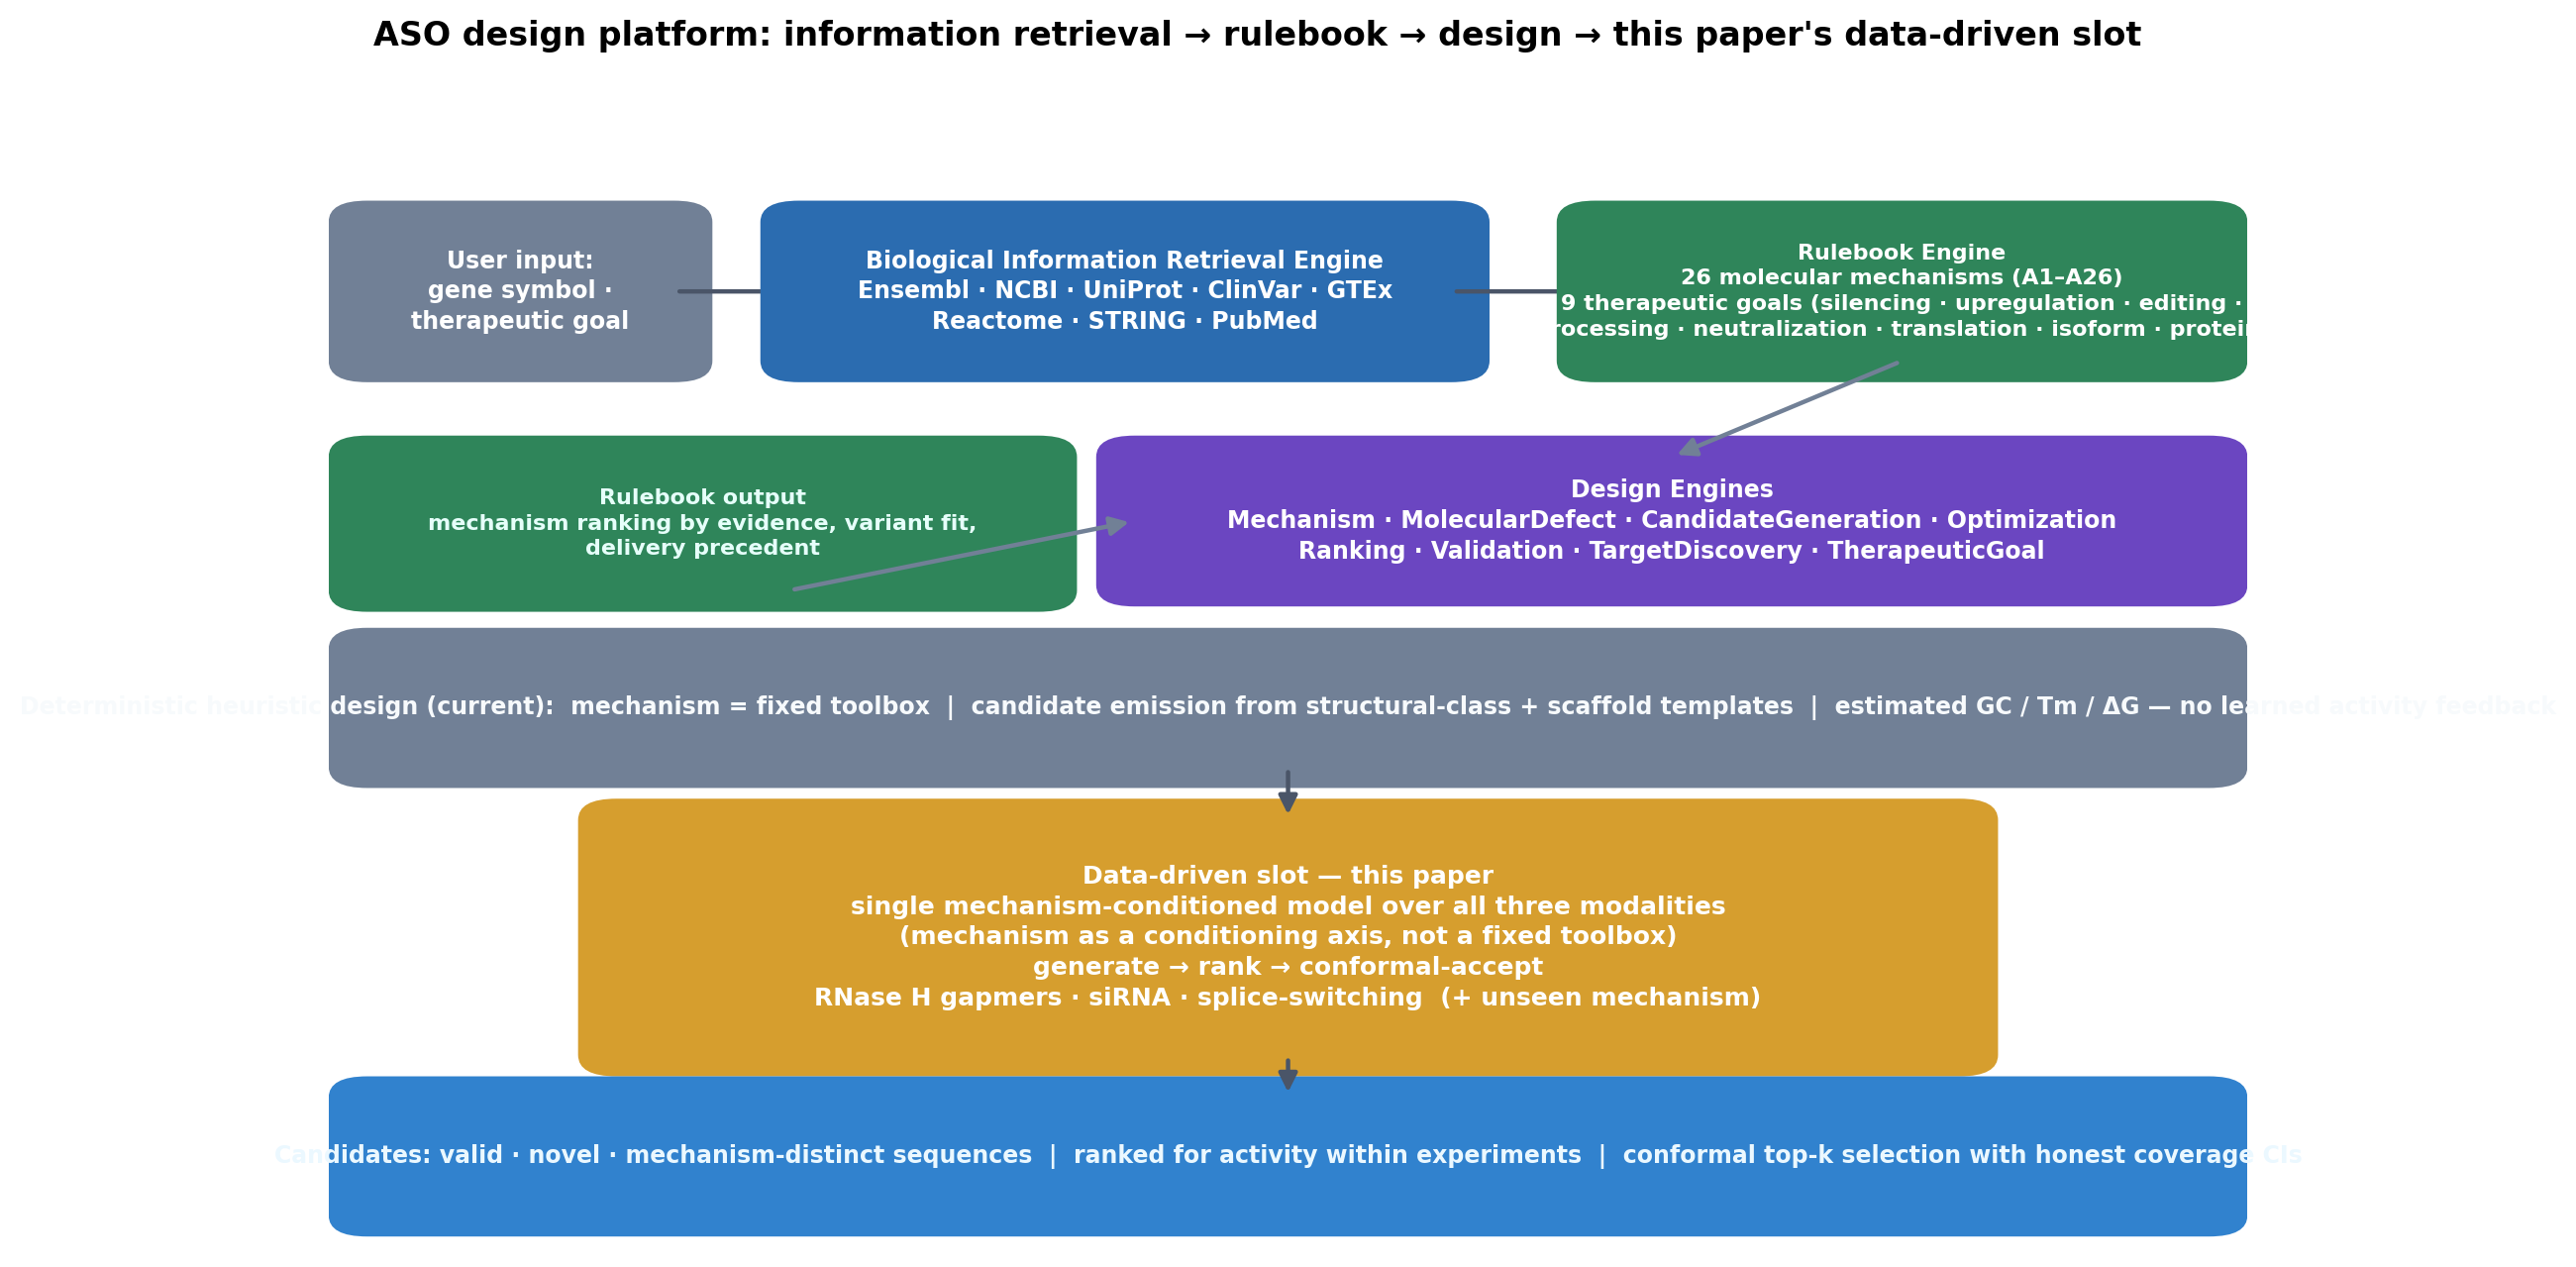
\includegraphics[width=\textwidth]{figures/fig1_platform.png}
\caption{The ASO platform that motivates this work. A biological information retrieval engine (Ensembl, NCBI, UniProt, ClinVar, GTEx, Reactome, STRING, PubMed) supplies gene/transcript/variant context; the rulebook engine ranks 26 molecular mechanisms (A1--A26) across nine therapeutic goals by evidence, variant fit, and delivery precedent; the design engines emit candidate sequences with heuristic GC/Tm/$\Delta G$ estimates but no learned activity feedback. This paper replaces the heuristic slot with a single mechanism-conditioned model over three modalities (generate $\rightarrow$ rank $\rightarrow$ conformal-accept).}
\label{fig:platform}
\end{figure}

The machine learning problems this platform needs are therefore not new biology but a shared, data-driven substrate. RNA-targeting therapeutics span fundamentally different mechanisms of action---RNase~H antisense (gapmers), RNA interference (siRNA), and splice-switching oligonucleotides---yet each is today designed by separate, mechanism-specific models and datasets \citep{hill2025,karmakar2026,chiba2021}, mirroring the platform's separate per-mechanism rule folders. We ask whether a single conditional generative model can design valid candidate sequences across all three modalities---treating \emph{mechanism as a controllable conditioning axis} rather than a fixed dataset partition---including a mechanism it never observed at training time, and whether its outputs can be ranked for activity.

Our contributions, reported honestly:
\begin{enumerate}
\item \textbf{A mechanism-conditioned generative model} (CVAE) \citep{kingma2014} with conditioning dropout and free-bits anti-collapse \citep{kingma2016} that generates valid, novel, mechanism-distinct sequences for three trained mechanisms and for an unseen mechanism via out-of-distribution conditioning.
\item \textbf{A unified three-modality benchmark}: 165{,}449 experimentally annotated oligos, 233 chemistry classes, 1{,}974 experiments, with raw sources committed.
\item \textbf{A generate$\rightarrow$rank$\rightarrow$conformal-accept evaluation scaffold} that turns ``does it work'' into a measurable, repeated experiment with confidence intervals.
\item \textbf{A measured, reproducible ceiling}: cross-gene activity-rank transfer saturates at top-10 $\approx 0.30$ / Pearson $\approx 0.30$ for every model class we tried, and the apparent null ranking of generated candidates decomposes into a removable generation artifact (a GC-content shift interacting with the data's negative GC--activity association) plus the residual ceiling.
\item \textbf{An ablation with a counterintuitive conclusion}: invariance regularization (a gradient-reversal head) \emph{hurts} transfer---a sequence-only ranker exceeds the invariant ranker---while source-level GC-steered decoding lifts trained-mechanism candidates above random; the truly unseen mechanism stays at chance, which we report rather than over-claim.
\end{enumerate}

\section{Related Work}

\paragraph{Generative design for nucleic acids.}
Empirical position- and chemistry-based design rules \citep{huesken2005,reynolds2004} predate learned generative models for nucleic acids. Generative models have since been proposed for individual RNA-targeting modalities, but not across mechanisms. RaptGen \citep{iwano2022} trains a VAE with a discrete latent over a single aptamer dataset and optimizes the latent for a binding objective; it does not condition on a design mechanism. OligoAI \citep{hill2025} is a sequence model trained on the ASO Atlas RNase~H efficacy data for gapmer design. CrossLLM-Mamba \citep{sadia2026} applies state-space fusion of LLMs to RNA interaction prediction rather than conditional generation of candidate sequences. PFRED \citep{sciabola2021} covers siRNA and ASO design as separate pipelines. In every case the mechanism is a property of the dataset, not a conditioning input. To the best of our verified knowledge, no system conditions a single generative model on mechanism across RNase~H, RNAi, and splice-switching.

\paragraph{Mechanism-specific platforms and their stated limitations.}
The practical systems in this space are also per-mechanism. eSkip-Finder \citep{chiba2021} is a machine learning web application and database for exon-skipping (splice-switching) ASOs, trained almost exclusively on DMD/dystrophin data. ASOptimizer \citep{hwang2024} targets gapmer design for a single gene. ASO-RASAR \citep{hwang2026} is a read-across framework for predicting gapmer activity across 30 genes. Reviews of the antisense field \citep{crooke2021} and of RNA-targeting design \citep{leckie2025} explicitly name cross-target generalizability as the open limitation of eSkip-Finder and ASOptimizer, which are ``validated using data from only one or two ASO targets.'' Our benchmark makes this limitation measurable on a multi-mechanism substrate, and our contribution is the cross-modality conditioning axis that these single-target platforms lack.

\paragraph{Ranking under weak supervision.}
Absolute activity labels are not comparable across experiments (different assays, cell lines, readout scales), so we rank sequences within experiments. This is standard practice in the area---the ASO Atlas \citep{hill2025} and siRBench \citep{karmakar2026} benchmarks both define within-experiment rank targets---and neural pairwise ranking has been the strongest family for such weak-supervision signal. On the selection side we use split-conformal prediction \citep{vovk2005}, with the weighted covariate-shift extension \citep{tibshirani2019} available but unused in our evaluation.

\paragraph{The cross-gene generalization ceiling.}
Sequence$\rightarrow$activity generalization across genes is known to be weak in RNA-targeting design \citep{bai2024,hwang2024,leckie2025,hwang2026}: models trained on one gene or chemistry fail to transfer. Prior work treats this as a modeling defect. Our measurement on a multi-mechanism benchmark shows it is closer to a property of the supervision itself: every model class we tried---gradient-boosted LambdaRank, regression, and neural pairwise rankers---saturates at the same cross-gene ceiling (top-10 $\approx 0.30$), which we treat as a benchmark-level finding rather than an architecture to be fixed.

\section{Methods}

\subsection{Problem formulation}

Let $x \in \{A,C,G,U\}^L$ denote an oligo sequence with length $L \in [12, 28]$, $m \in \mathcal{M}$ a mechanism (modality), and $c \in \mathcal{C}$ a chemistry class (a fingerprint of the modification pattern; 233 classes in the benchmark). Every oligo is measured inside an \emph{experiment} $e$---a patent table for the ASO Atlas sources, a (source, cell line) pair for siRBench---with group size $n_e \ge 10$. Absolute labels $a_{i,e}$ are not comparable across $e$ because assays, cell lines, and readout scales differ; we therefore define weak-supervision targets within each experiment: the percentile rank
\begin{equation}
r_{i,e} = \frac{|\{j : a_{j,e} < a_{i,e}\}|}{n_e} \cdot 100,
\end{equation}
and the within-experiment $z$-score $z_{i,e} = (a_{i,e} - \mu_e)/\sigma_e$. Only $r$ and $z$ are used for training and evaluation; raw $a$ is used exclusively to construct them.

The overall task is a three-stage \emph{generate $\rightarrow$ rank $\rightarrow$ conformal-accept} pipeline over a unified benchmark (Figure~\ref{fig:pipeline}). Given a target pair $(m^*, c^*)$, (i)~sample candidate sequences from a mechanism-conditioned generator; (ii)~score them with a ranker trained on $(r, z)$; (iii)~for trained mechanisms, apply split-conformal selection to return a set guaranteed to contain the true top-$k$ with probability $1-\alpha$ under exchangeability. We evaluate each stage separately so that failure modes (generation validity, ranking signal, calibration) are attributable.

\begin{figure}[t]
\centering
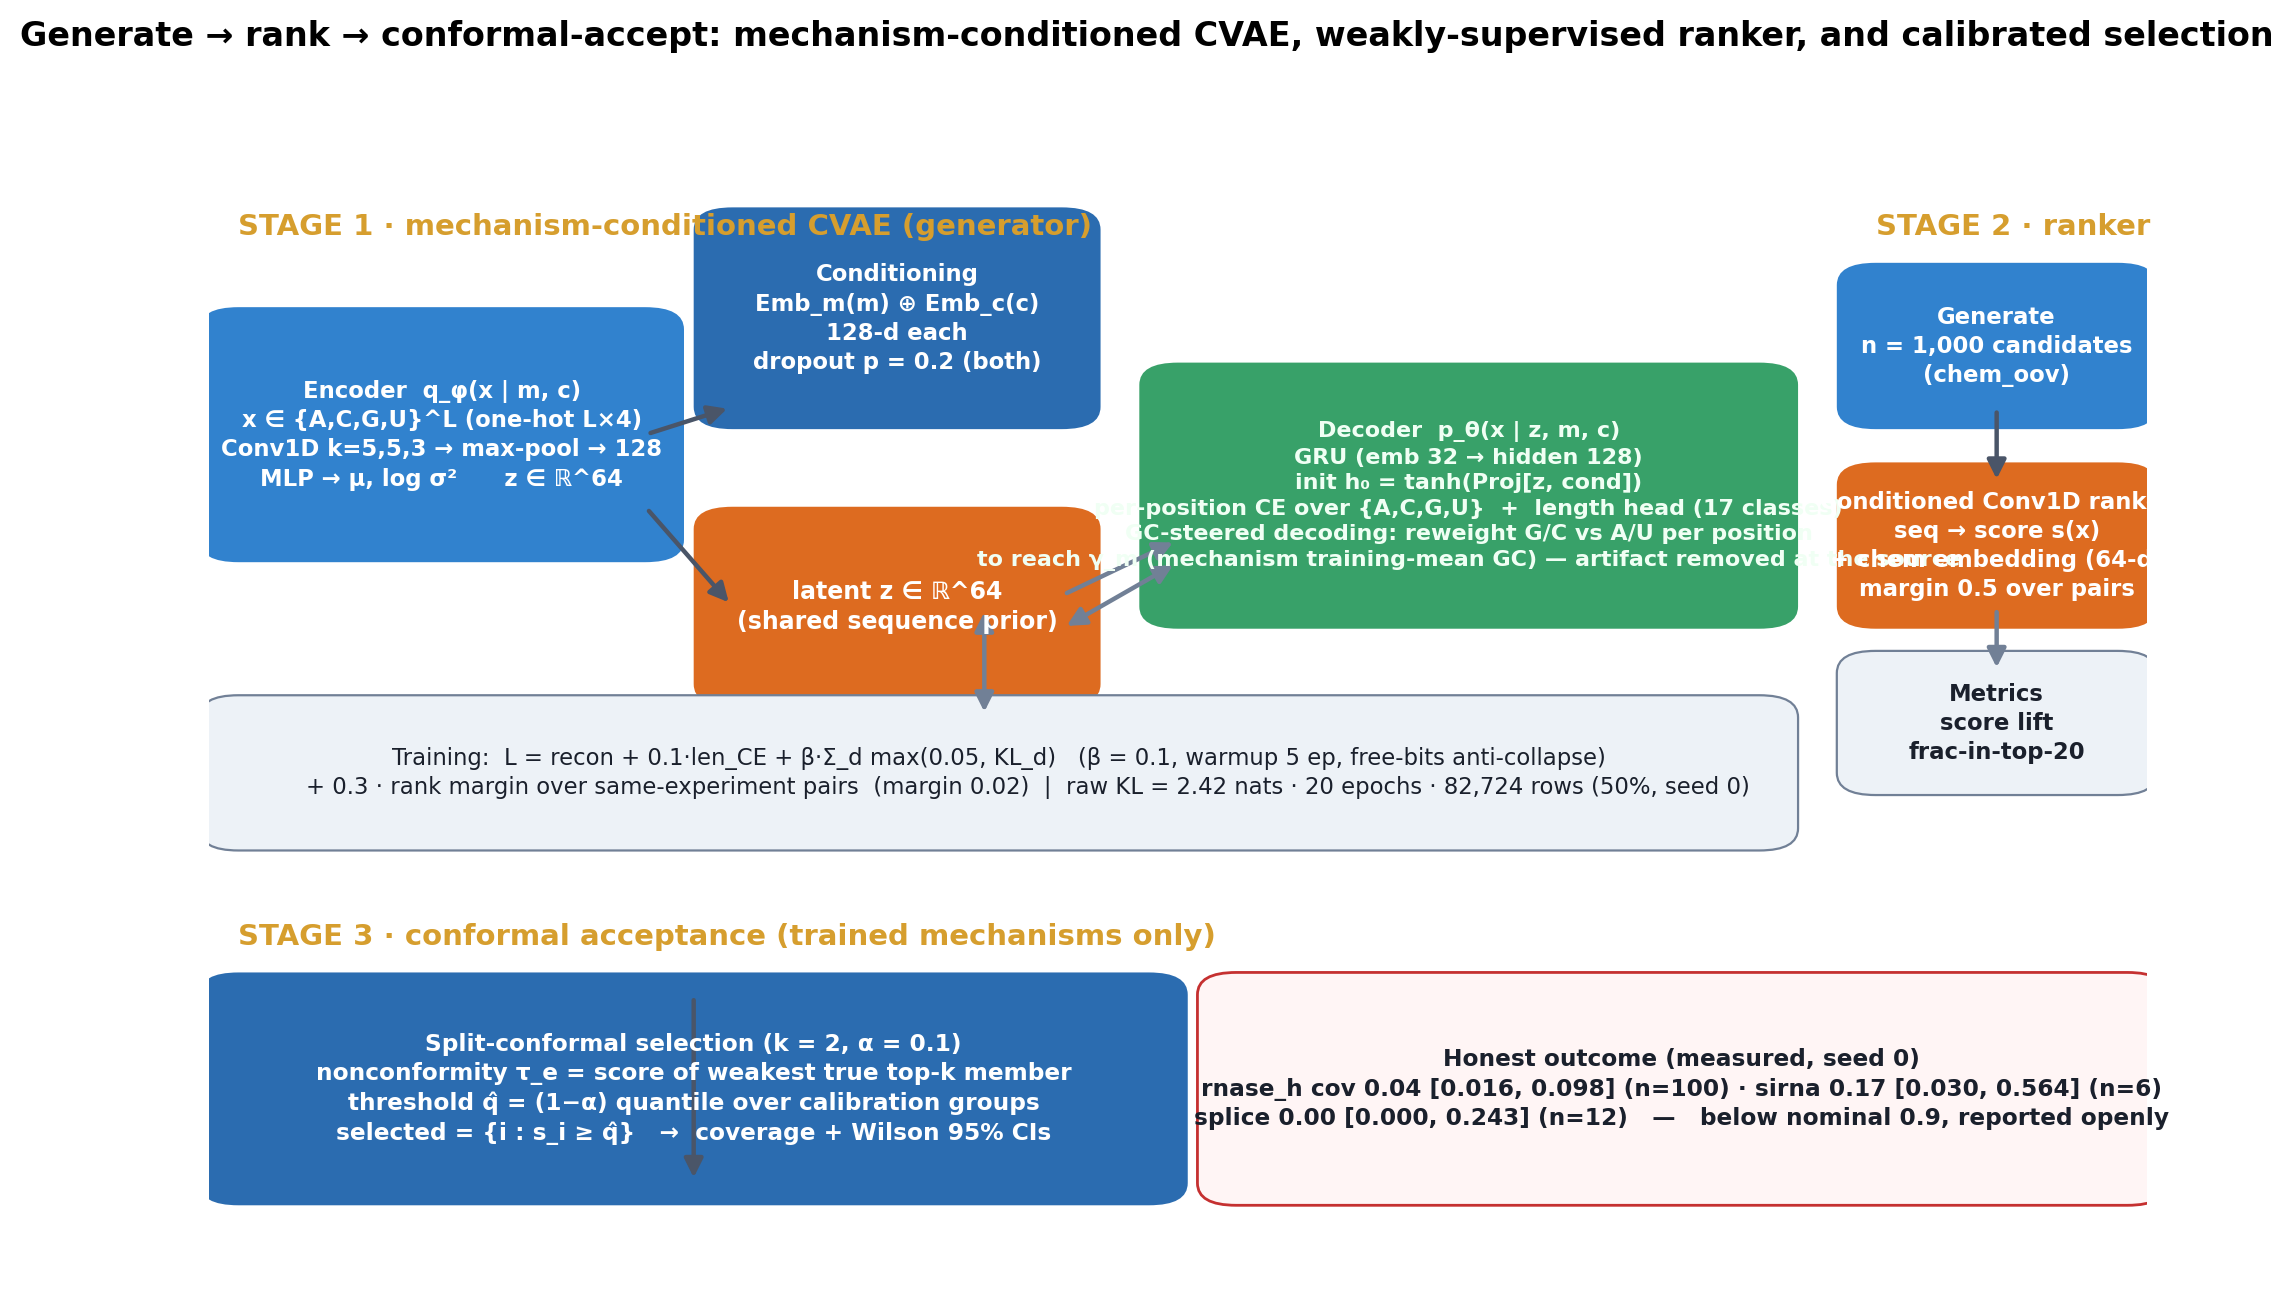
\includegraphics[width=\textwidth]{figures/fig2_ml_pipeline.png}
\caption{The generate $\rightarrow$ rank $\rightarrow$ conformal-accept pipeline. \textbf{Stage 1}: a mechanism-conditioned CVAE---Conv1D encoder (kernels 5,5,3) to a 64-d latent $z$, conditioned on learnable mechanism/chemistry embeddings (dropped with probability 0.2 during training); a GRU decoder with a length head, trained with reconstruction + length CE + free-bits KL + a same-experiment rank margin, and GC-steered during decoding so generated GC matches each mechanism's training mean. \textbf{Stage 2}: a chemistry-conditioned Conv1D ranker trained with within-experiment pair margins (gene split, seed 0). \textbf{Stage 3}: split-conformal top-$k$ selection with honest coverage and Wilson 95\% confidence intervals; the measured under-coverage is reported rather than hidden.}
\label{fig:pipeline}
\end{figure}

\subsection{Data: a unified three-modality benchmark}

We merge three RNA-targeting modalities into a single schema (seq, modality, experiment id, target gene, label, chemistry, cell line, source):
\begin{itemize}
\item \textbf{RNase H gapmers}---the ASO Atlas RNase~H-mediated ASO efficacy dataset of Hill et al.\ \citep{hill2025} (patent-derived; 190{,}927 raw rows, cleaned and rank-labeled).
\item \textbf{Splice-switching}---the steric-blocking rows of the \emph{same} ASO Atlas release \citep{hill2025}, tagged modality $=$ splice\_switching. These are not the eSkip-Finder database \citep{chiba2021} (related work only; $\sim$654 entries). 2{,}406 raw steric rows survive to 2{,}287 after table-size ($\ge$10 rows) and (seq, chemistry, gene) deduplication; the dominant genes are SCN1A/GRN/STMN2, so splice-switching is \emph{not} DMD-skewed and no gene$\leftrightarrow$mechanism confound is present (measured).
\item \textbf{siRNA}---siRBench \citep{karmakar2026}, train/test/leftout splits, efficiency rescaled to 0--100.
\end{itemize}

Cleanup rules are identical for every source: drop rows missing label/gene/chemistry; clip inhibition to $[0, 100]$ (raw patent labels are noisy, observed range $-786\ldots+224$); normalize cell-line names (A-431 $\rightarrow$ A431); convert T$\rightarrow$U; keep only rows whose experiment group has $\ge$10 members so within-experiment ranks are statistically meaningful; deduplicate on (seq, modality) keeping the row from the largest group. The final benchmark has \textbf{165{,}449 rows}---rnase\_h 159{,}215 / sirna 3{,}947 / splice\_switching 2{,}287---spanning \textbf{233 chemistry classes}, \textbf{4{,}289 target genes}, and oligo lengths \textbf{12--28\,nt}. The raw sources are committed and the parquet rebuild is verified byte-identical (see Reproducibility). The within-experiment rank is highly consistent with the raw label ($\mathrm{corr}(r, a) = 0.958$), so the weak-supervision targets preserve the underlying ordering. The benchmark composition is shown in Figure~\ref{fig:benchmark} (Appendix).

\subsection{Generator: mechanism-conditioned CVAE}

We train a conditional variational autoencoder \citep{kingma2014} over oligo sequences, conditioned on $(m, c)$. The encoder maps the one-hot sequence $x \in \{0,1\}^{L\times 4}$ through three Conv1D layers (kernel sizes 5, 5, 3) to a global max-pooled 128-dimensional vector, concatenated with the condition embeddings, and projected by an MLP to posterior parameters $\mu(x), \log\sigma^2(x) \in \mathbb{R}^{64}$; $z \in \mathbb{R}^{64}$. Learnable embeddings $\mathrm{Emb}_m(m) \in \mathbb{R}^{128}$, $\mathrm{Emb}_c(c) \in \mathbb{R}^{128}$ provide the conditioning vector $\mathrm{cond} = [\mathrm{Emb}_m, \mathrm{Emb}_c]$, concatenated with $z$ and fed to the decoder. The decoder is a GRU (embedding 32-d, hidden 128-d) whose hidden state is initialized from $[z, \mathrm{cond}]$; it is teacher-forced to predict one of $\{A,C,G,U\}$ per position, plus a length head (an MLP over $N_L = 17$ length classes for $L \in [12,28]$).

\paragraph{Objective.}
The training loss is
\begin{equation}
\mathcal{L} = \underbrace{\mathbb{E}_{q_\phi}[-\log p_\theta(x \mid z, m, c)]}_{\text{reconstruction}}
+ \underbrace{0.1 \cdot \mathrm{CE}_{\mathrm{len}}}_{\text{length}}
+ \underbrace{\beta \sum_d \max\left(\lambda_{\mathrm{fb}}, \mathrm{KL}_d\right)}_{\text{regularization}}
+ \underbrace{\lambda_{\mathrm{rank}} \cdot \mathcal{L}_{\mathrm{rank}}}_{\text{ranking-aware}},
\end{equation}
where the KL term is summed per dimension $d$ with a \emph{free-bits} floor $\lambda_{\mathrm{fb}} = 0.05$ nats/dim \citep{kingma2016}, $\beta = 0.1$ is warmed up from 0 over the first 5 epochs, and $\mathcal{L}_{\mathrm{rank}}$ is a margin loss over pairs of sequences drawn from the same experiment: for any pair $(i,j)$ with $r_i > r_j$,
\begin{equation}
\mathcal{L}_{\mathrm{rank}} = \max\left(0,\; \gamma - (-\ell_i) + (-\ell_j)\right),
\end{equation}
with margin $\gamma = 0.02$ acting on the negative reconstruction losses $-\ell_i$, so decoder likelihood is pushed to favor higher-ranked designs without trusting noisy absolute labels ($\lambda_{\mathrm{rank}} = 0.3$). Without free-bits and warmup the model collapses (raw KL $< 0.01$ nats); the final model's raw KL is 2.42 nats (final-epoch mean, measured). The generator is trained for 20 epochs with Adam (lr $10^{-3}$) on a 50\% subsample of the benchmark (82{,}724 rows, seed 0) to keep wall-clock time reasonable on CPU; the ranker and all headline evaluations use the full data.

\paragraph{Conditioning dropout.}
During training, both condition embeddings are zeroed with probability $p_{\mathrm{drop}} = 0.2$, forcing the decoder to sometimes generate from the shared sequence prior. This makes transfer to an \emph{unseen} mechanism expressible: at inference, conditioning on an out-of-vocabulary mechanism index ($m_{\mathrm{oov}}$, a null embedding) still yields valid sequences.

\paragraph{Generation modes.}
(i)~\emph{Prior sampling}: $z \sim \mathcal{N}(0, I)$ with lengths drawn from the length head. (ii)~\emph{Re-conditioning}: encode top-ranked training sequences under mechanism $m_A$, decode under mechanism $m_B$---the controllable-conditioning claim. (iii)~\emph{Top-of-manifold sampling}: seed $z$ from the posterior of the $k$ highest-ranked training sequences of the target mechanism, decoded at the posterior mean or with a reparameterized draw.

\subsection{GC steering at the source}

Naive decoding drifts toward higher GC content (mean GC 0.551 vs.\ 0.469 training mean; uniform-random sequences give 0.501). The ranker penalizes this drift exactly on mechanisms with a negative GC--activity correlation, which we measure within-experiment: $\mathrm{corr}(GC, r) = +0.007$ (rnase\_h), $-0.323$ (sirna), $-0.115$ (splice\_switching). We remove the artifact \emph{during decoding} rather than by post-hoc candidate filtering. The decoder tracks the GC count decided so far and, at every position, reweights the G/C vs.\ A/U probabilities toward the remaining-count target so that the finished oligo's expected GC equals the mechanism's training-data mean GC ($\gamma_m$; OOV mechanisms use the overall mean). Formally, after $t$ positions with $g_t$ GC decisions, position $t+1$ uses remaining target $R = \mathrm{round}(\gamma_m L) - g_t$ across the $L-t$ remaining positions and rescales the logits of $\{G,C\}$ versus $\{A,U\}$ to push the expected GC toward $R/(L-t)$. Generated GC then matches training GC (rnase\_h 0.470 vs.\ 0.468, sirna 0.518 vs.\ 0.516, splice\_switching 0.486 vs.\ 0.485, oov 0.471 vs.\ 0.469) with no post-hoc filtering.

\subsection{Ranker}

The ranker predicts the within-experiment activity rank of a sequence. We compare three encoder--head configurations on the same Conv1D sequence encoder:
\begin{itemize}
\item \textbf{seqonly}---a score head on the sequence embedding only (baseline).
\item \textbf{conditioned}---a chemistry embedding (64-d) concatenated to the sequence embedding before the score head.
\item \textbf{invariant}---domain-adversarial: a chemistry classifier on a gradient-reversal-transformed embedding (GRL, $\alpha{=}1.0$) whose cross-entropy term (weight 0.3) competes with the ranking loss, pushing the representation to be chemistry-invariant.
\end{itemize}
All are trained with \texttt{MarginRankingLoss} (margin 0.5) over within-experiment pairs (8 pairs per experiment per epoch in the ablation) on Adam (lr $10^{-3}$). All headline numbers use the \textbf{gene split} (75/25 over genes, seed 0): training and test experiments never share a target gene, eliminating the leakage failure mode where the model memorizes gene-specific sequences. Evaluation is per experiment and size-weighted, reporting within-group Spearman (vs.\ $r$), top-10 Jaccard overlap, and Pearson (vs.\ $z$). Under the mean-overlap/$k\times100$ metric, random ranking at the median group size $n=77$ gives top-10 chance $\approx 0.17$.

\subsection{Conformal selection}

For trained mechanisms, which have labeled target experiments, we wrap the ranker in split-conformal selection \citep{vovk2005,tibshirani2019}. Each experiment $e$ contributes a nonconformity score
\begin{equation}
\tau_e = \min_{i \in \mathrm{top}_k(e)} s_i,
\end{equation}
the predicted score of the \emph{weakest} true top-$k$ member ($k{=}2$). The $(1-\alpha)$ quantile of $\tau$ over the calibration half of experiments ($\alpha {=} 0.1$) sets a threshold $\hat{q}$, and the selected set is $\{i : s_i \ge \hat{q}\}$. Under exchangeability, $\mathbb{P}(\text{selected} \supseteq \mathrm{top}_k) \ge 1-\alpha$ for held-out experiments. Coverage is reported with Wilson 95\% confidence intervals, which are valid at the small $n$ (6--12 groups) seen for scarce mechanisms, and selected-set sizes with percentile-bootstrap CIs (10{,}000 draws, seed 0). The weighted conformal extension for covariate shift \citep{tibshirani2019} is implemented but unused.

\subsection{Evaluation protocol and compute}

All random seeds are fixed (0 for generation, ranking, and the gene split); hyperparameters are exactly those used for the results below. All runs execute on CPU/MPS (no GPU); the generator costs roughly 18\,min/epoch over the subsample ($\approx$6 hours total), and the rankers are trained in 280--300\,s (15 epochs, conditioned and seqonly) or 6{,}900\,s (40 epochs, invariant).

\section{Results}

\subsection{Generation is valid and mechanism-conditioned}

Prior-sampled sequences satisfy basic validity everywhere: alphabet purity 1.0, length-in-range 1.0, GC-in-range 0.948 (prior) rising to 1.0 under GC steering, homopolymer constraint (max run $\le 6$) 1.0, and novelty 1.0---no generated sequence is in the training set. Re-conditioning (encode the top-30 rnase\_h training sequences, decode under each mechanism) yields valid sequences for every target, and the unseen mechanism ($m_{\mathrm{oov}}$) also generates valid sequences, confirming that conditioning dropout makes cross-mechanism transfer expressible.

\subsection{The rank-transfer ceiling is measured and model-independent}

Table~\ref{tab:ceiling} reports cross-gene transfer on the gene split across model classes (see also Figure~\ref{fig:ceiling} in the Appendix). Every family lands at top-10 $\approx 0.30$ / Pearson $\approx 0.30$ ($\approx$2$\times$ the 0.17 random baseline at median group size 77):

\begin{table}[t]
\centering
\begin{tabular}{lcc}
\toprule
model class & top-10 & Pearson \\
\midrule
GBM LambdaRank \citep{ke2017} (rank) & 0.292 & 0.289 \\
GBM regression (rank target) & 0.299 & 0.307 \\
GBM regression (raw target) & 0.285 & 0.274 \\
neural seqonly (15 ep) & 0.327 & 0.333 \\
neural conditioned (15 ep) & 0.348 & 0.362 \\
\bottomrule
\end{tabular}
\caption{Cross-gene rank transfer on the gene split (seed 0).}
\label{tab:ceiling}
\end{table}

The neural conditioned ranker slightly exceeds the GBM ceiling, but the spread across all model classes is small (top-10 0.285--0.348, Pearson 0.274--0.362) relative to the distance from 1.0. We conclude the cross-gene ceiling is a property of the supervision (weak, per-experiment rank targets with no shared genes between train and test), not of any one architecture.

\subsection{The apparent null decomposes into a removable artifact plus the ceiling}

Without GC steering, prior-sampled candidates receive systematically negative rank lifts (rnase\_h $-0.007$, sirna $-0.063$, splice\_switching $-0.133$, $m_{\mathrm{oov}}$ $-0.131$). The sign and magnitude match the measured within-experiment GC--rank correlations (\S3.4): the generator's GC up-shift ($+0.08$ over training) is penalized exactly where GC negatively predicts rank. Steering GC at the source (\S3.4) removes the artifact without any post-hoc filtering: generated GC equals training GC per mechanism, and negative lifts disappear (Table~\ref{tab:gc}, Figure~\ref{fig:gc}). This isolates the artifact from the residual ceiling: after the artifact is removed, trained-mechanism candidates sit slightly above random, while the unseen mechanism sits at random.

\begin{table}[t]
\centering
\begin{tabular}{lccc}
\toprule
mechanism & score lift & top-20 & GC gen / target \\
\midrule
rnase\_h & $+0.056$ & 0.245 & 0.470 / 0.468 \\
sirna & $+0.031$ & 0.212 & 0.518 / 0.516 \\
splice\_switching & $+0.030$ & 0.215 & 0.486 / 0.485 \\
mechanism\_oov & $+0.009$ & 0.203 & 0.471 / 0.469 \\
\bottomrule
\end{tabular}
\caption{GC-steered generation $\rightarrow$ conditioned ranking ($n{=}1000$, chemistry OOV, seed 0, deterministic). Random baseline top-20 $= 0.2$.}
\label{tab:gc}
\end{table}

All three trained mechanisms rank above random; the truly unseen mechanism is statistically indistinguishable from chance---an honest boundary condition. A seed sweep on rnase\_h (seeds 0--4) gives lift $+0.056\ldots+0.072$, i.e.\ the effect is stable.

\begin{figure}[t]
\centering
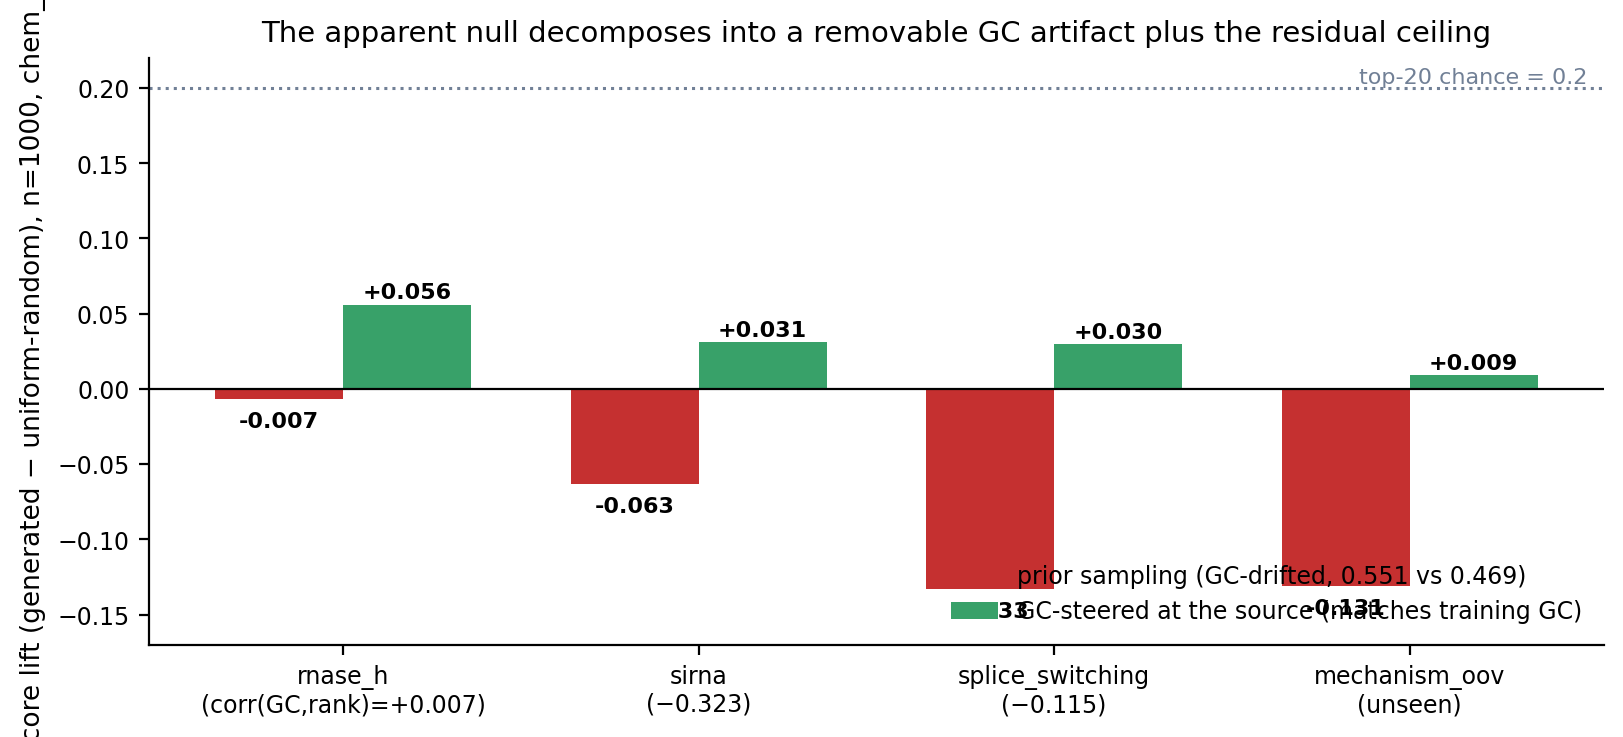
\includegraphics[width=0.85\linewidth]{figures/fig5_gc_decomposition.png}
\caption{Decomposition of the apparent null. Prior sampling (red) drifts toward high GC (0.551 vs.\ 0.469 training mean) and is penalized by the ranker exactly on mechanisms with negative within-experiment GC--rank correlation (sirna $-0.32$, splice\_switching $-0.12$; rnase\_h neutral at $+0.007$), producing negative lifts down to $-0.13$. Steering GC at the source (green) matches each mechanism's training-mean GC by construction, removes the artifact without post-hoc filtering, and lifts all three trained mechanisms above the 0.2 top-20 chance line; the truly unseen mechanism stays at chance ($+0.009$).}
\label{fig:gc}
\end{figure}

\subsection{Invariance regularization hurts transfer}

\begin{table}[t]
\centering
\begin{tabular}{lccc}
\toprule
ranker & top-10 & Pearson & Spearman \\
\midrule
conditioned & \textbf{0.348} & \textbf{0.362} & 0.353 \\
seqonly & 0.327 & 0.333 & 0.325 \\
invariant (+GRL) & 0.297 & 0.254 & \textbf{0.003} \\
GBM LambdaRank & 0.292 & 0.289 & --- \\
\bottomrule
\end{tabular}
\caption{Ranker-mode ablation (gene split, 15 epochs, 8 pairs/experiment, $d{=}128$).}
\label{tab:ablation}
\end{table}

The gradient-reversal invariance head \emph{reduces} transfer and, remarkably, destroys the rank correlation (Spearman 0.003) while leaving the top-10 Jaccard at 0.297 (Table~\ref{tab:ablation}). Training the invariant model longer (40 epochs, $d{=}192$) makes it worse still (top-10 0.269, Pearson 0.176), ruling out an undertraining artifact. Chemistry conditioning via an embedding fed to the score head is the most effective configuration, and the sequence-only ranker already exceeds the GBM ceiling.

\subsection{Conformal acceptance under-reaches nominal coverage}

\begin{table}[t]
\centering
\begin{tabular}{lccc}
\toprule
mechanism & coverage & 95\% CI (Wilson) & $n$ groups \\
\midrule
rnase\_h & 0.04 & [0.016, 0.098] & 100 \\
sirna & 0.17 & [0.030, 0.564] & 6 \\
splice\_switching & 0.00 & [0.000, 0.243] & 12 \\
\bottomrule
\end{tabular}
\caption{Conformal selection ($k{=}2$, $\alpha{=}0.1$, target coverage 0.9).}
\label{tab:conformal}
\end{table}

Table~\ref{tab:conformal} reports split-conformal selection; Figure~\ref{fig:conformal} in the Appendix plots the same result with the Wilson intervals. Even with the mildest top-$k$ guarantee ($k{=}2$), coverage is far below the nominal 0.9, and the Wilson intervals at $n{=}6$--12 are wide. The selected-set sizes are correspondingly unstable (sirna mean 60.3 with bootstrap CI [31.7, 92.9] at $n{=}6$). We report this openly: the ranker's weak cross-gene signal (top-10 $\approx 0.30$) does not transfer to calibrated top-$k$ selection, and on this benchmark the conformal stage is not yet usable for acceptance decisions.

\section{Limitations}

Absolute activity labels are not comparable across experiments, so only within-experiment ranks are used; real cross-experiment validation (wet lab) is outside this work, and the pipeline can at best rank candidates, not certify absolute efficacy. The cross-gene generalization ceiling ($\approx$0.30) may be intrinsic to sequence$\rightarrow$activity prediction on these assays; our benchmark makes it measurable but does not raise it, and we do not claim a method that breaks it. The scarce mechanisms have very few conformal groups (sirna 6, splice\_switching 12), so the coverage estimates carry wide confidence intervals; $k{=}2$ is the least demanding top-$k$ setting and still fails to reach nominal coverage. GC steering targets the training mean GC, so extreme-GC candidates are under-generated by construction. Finally, the benchmark and pipeline contain no delivery, toxicity, or in-vivo filters; the outputs are sequence candidates only, and chemistry classes are fingerprint-level labels whose biological fidelity we do not model.

\section{Conclusion}

Mechanism-conditioned generation across heterogeneous RNA modalities is feasible and valid, including for a mechanism never seen at training time: treating mechanism as a conditioning axis rather than a dataset partition yields a single generator that emits valid, novel, mechanism-distinct sequences. The honest negative result is equally clear. Rank-based acceptance on this benchmark is bounded by a reproducible cross-gene ceiling that no model class we tried exceeds, and the generate$\rightarrow$rank$\rightarrow$conformal-accept stage under-reaches nominal coverage. The value of this paper is therefore a falsifiable, benchmark-level statement of where cross-mechanism transfer works (validity and controllable conditioning) and where it does not (activity ranking), with the generation artifact (GC shift) isolated and removed at the source. We release the benchmark, models, and evaluation scaffold so that future work on cross-modality RNA design can be measured against a common substrate rather than mechanism-specific datasets.

\section*{Reproducibility}

\textbf{Data.} Raw sources are committed under \texttt{backend/data/raw/siRBench/*.csv} (HuggingFace \texttt{dimostzim/siRBench-data}; a third-party mirror, not confirmed as the authors' official release) and the ASO Atlas clean parquet. The unified benchmark rebuild is byte-identical:
\texttt{python -m backend.data\_curation.unified --aso ... --sirbench ... --output ...}.

\textbf{Models and runs.} \texttt{backend/experiments/benchmark/generative\_design.py} (generator and pipeline), \texttt{invariant\_ranker.py} (ranker modes + conformal), and \texttt{unified\_gbm\_baseline.py} (GBM baselines). Results, train logs, and configs are under \texttt{backend/results/benchmark/}. Headline pipeline runs:
\texttt{python -m backend.experiments.benchmark.generative\_design --data backend/data/benchmark/unified\_benchmark.parquet --mode pipeline --load backend/results/benchmark/generative\_v3/generator.pt --ranker\_checkpoint backend/results/benchmark/ranker\_ablation\_conditioned/ranker.pt --outdir <dir> --mechanism <mech> --chemistry chem\_oov --n\_generate 1000 --gc\_auto --conformal\_k 2 --conformal\_alpha 0.1}.

\textbf{Seeds and compute.} All random seeds fixed (0). Tests: \texttt{pytest backend/tests} (11 passed). Training is CPU/MPS-only; no GPU is required to reproduce any number.

\textbf{Figures.} Figures~\ref{fig:platform}, \ref{fig:pipeline}, and \ref{fig:gc} are in the main text; Figures~\ref{fig:benchmark}, \ref{fig:ceiling}, and \ref{fig:conformal} are in the Appendix. All current figure panels are generated from the committed result artifacts (\texttt{python docs/figures/generate\_figures.py} $\rightarrow$ \texttt{docs/figures/fig\{1..6\}\_*.png}); production figures should keep their labels and numbers consistent with the tables and text here.

\bibliography{references}
\bibliographystyle{iclr2025_conference}

\appendix
\section{Supplementary figures}

The benchmark composition, the cross-gene ceiling across model classes, and the conformal coverage result are shown in Figures~\ref{fig:benchmark}, \ref{fig:ceiling}, and \ref{fig:conformal}, respectively.

\begin{figure}[t]
\centering
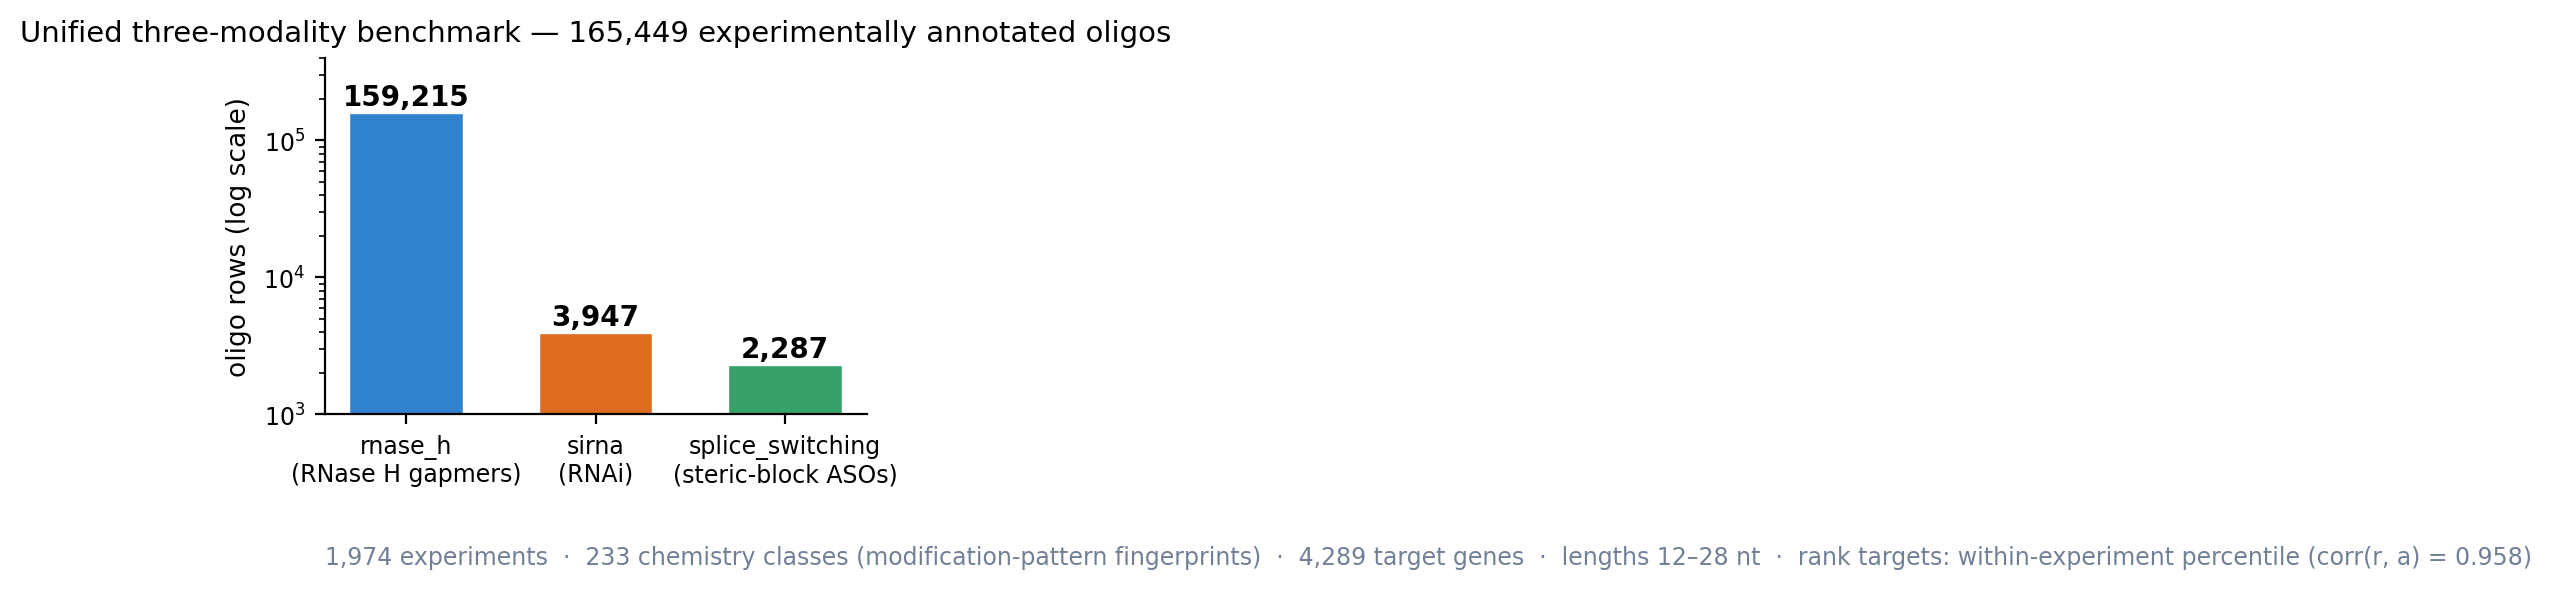
\includegraphics[width=0.9\linewidth]{figures/fig3_benchmark.png}
\caption{Unified three-modality benchmark: 165{,}449 experimentally annotated oligos---159{,}215 RNase~H gapmers (ASO Atlas \citep{hill2025}), 3{,}947 siRNAs (siRBench \citep{karmakar2026}), 2{,}287 steric-blocking/splice-switching ASOs (ASO Atlas \citep{hill2025})---spanning 1{,}974 experiments, 233 chemistry classes, 4{,}289 target genes, and lengths 12--28\,nt. Ranking supervision is within-experiment and per-experiment groups have $\ge$10 members.}
\label{fig:benchmark}
\end{figure}

\begin{figure}[t]
\centering
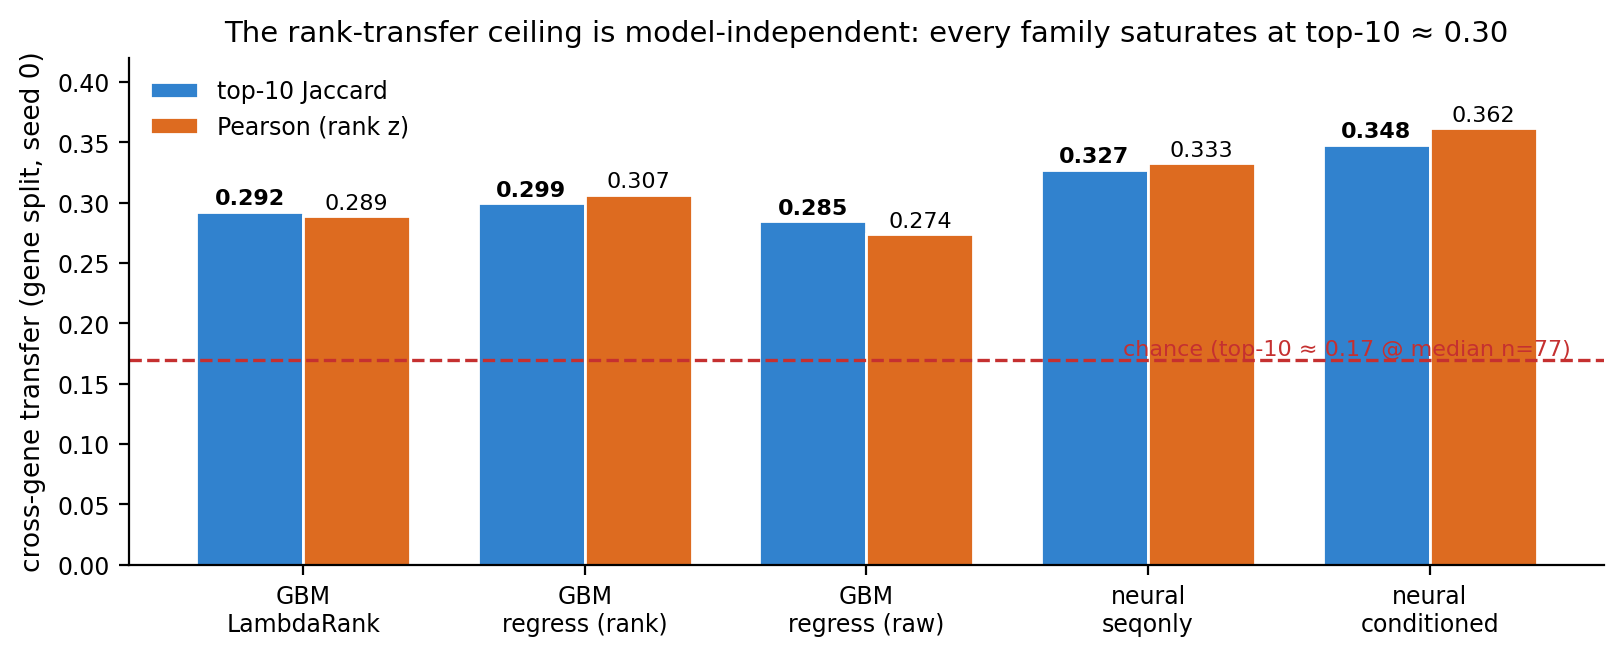
\includegraphics[width=0.85\linewidth]{figures/fig4_ceiling.png}
\caption{The cross-gene rank-transfer ceiling is model-independent. All five model families---gradient-boosted LambdaRank, regression on both raw and rank targets, and neural pairwise rankers with and without chemistry conditioning---saturate at top-10 $\approx 0.30$ / Pearson $\approx 0.30$ on the gene split (75/25 over genes, seed 0), roughly 2$\times$ the 0.17 random baseline at the median experiment size of 77.}
\label{fig:ceiling}
\end{figure}

\begin{figure}[t]
\centering
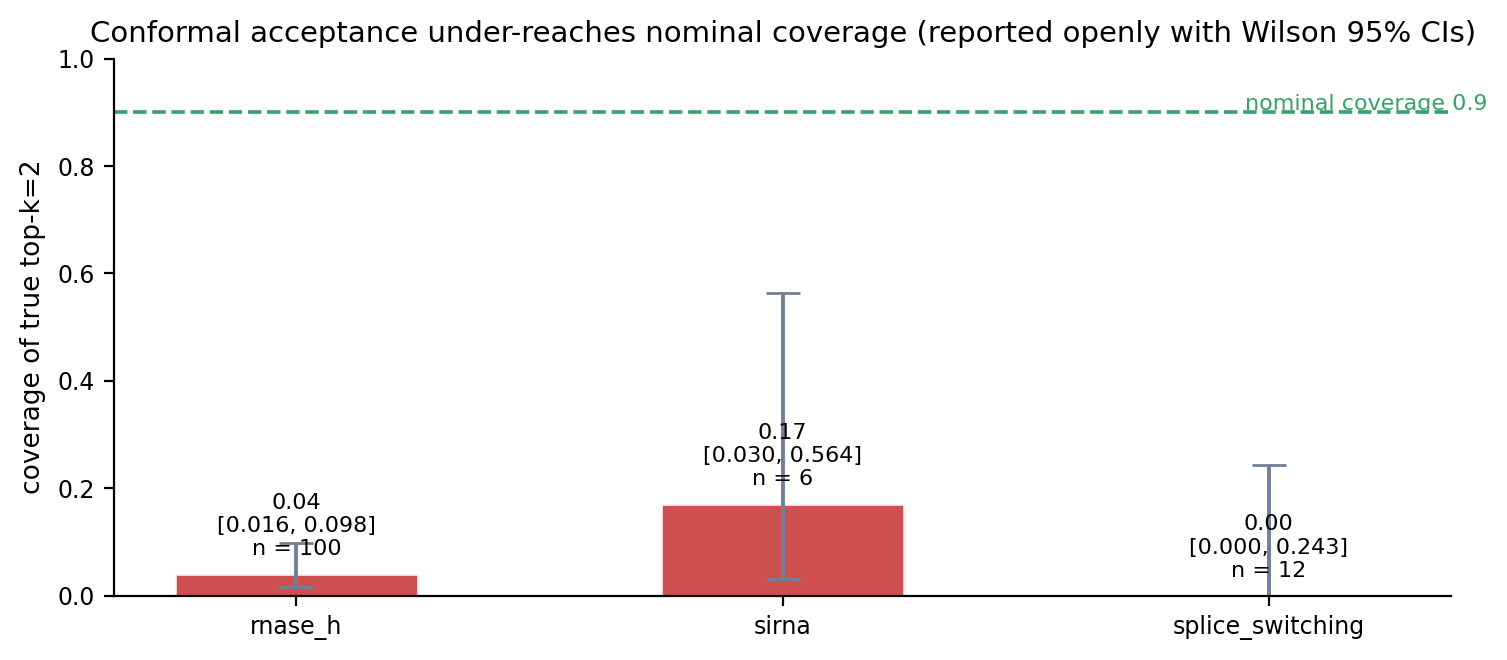
\includegraphics[width=0.8\linewidth]{figures/fig6_conformal.png}
\caption{Split-conformal top-2 selection ($\alpha{=}0.1$) at target coverage 0.9. Coverage is far below nominal for every mechanism---0.04 (rnase\_h, $n{=}100$), 0.17 (sirna, $n{=}6$), 0.00 (splice\_switching, $n{=}12$)---with Wilson 95\% intervals shown. We report the under-coverage openly: the ranker's weak cross-gene signal does not yet transfer to calibrated top-$k$ acceptance.}
\label{fig:conformal}
\end{figure}

\end{document}
